\documentclass{beamer}[10]
\usepackage{pgf}
\usepackage{beamerthemesplit}
\usepackage{array}
\usepackage{wrapfig}
\usepackage{varwidth}
%\usepackage{enumitem}
\usepackage{listings}
\lstset{language=bash,
	basicstyle=\ttfamily\scriptsize,		
	keywordstyle=\color{blue}\ttfamily,
	morekeywords={peter@kbpet},
	alsoletter={:~$},
	morekeywords=[2]{peter@kbpet:},
	keywordstyle=[2]{\color{red}},
	literate={\$}{{\textcolor{red}{\$}}}1 
	{:}{{\textcolor{red}{:}}}1
	{~}{{\textcolor{red}{\textasciitilde}}}1,
	breaklines=true,
	numbers=none,
	numbersep=5pt,
	stepnumber=1
}

%\usepackage{natbib}
\bibliographystyle{apalike}

\definecolor{kugreen}{RGB}{50,93,61}
\definecolor{kugreenlys}{RGB}{132,158,139}
\definecolor{kugreenlyslys}{RGB}{173,190,177}
\definecolor{kugreenlyslyslys}{RGB}{214,223,216}
\definecolor{kublue}{RGB}{0,101,163}
\definecolor{kubluelys}{RGB}{132,158,139}
\definecolor{kubluelyslys}{RGB}{173,190,177}
\definecolor{kubluelyslyslys}{RGB}{214,223,216}
\setbeamercovered{transparent}
\mode<presentation>
\usetheme[numbers,totalnumber,compress,sidebarshades]{PaloAlto}
%\setbeamertemplate{footline}[frame number]

\usecolortheme[named=kublue]{structure}
\useinnertheme{circles}
\usefonttheme[onlymath]{serif}
\setbeamercovered{transparent}
\setbeamertemplate{blocks}[rounded][shadow=true]

\logo{
\includegraphics[width=1.5cm]{gfx/eth_logo_kurz_pos}}
\title{Semester Project}
\subtitle{Mobile datalogger for recording decentrally captured dynamic motor vehicle data}
\author{Andreas Ziegler}
\institute{Advanced Iteractive Technologies \\ ETH Zürich}
\date{13th of July 2016}

\newcommand{\setlistspacing}[2]{\def\@ld{#1}\expandafter\def\csname
	@list\romannumeral\@ld \endcsname{\leftmargin\csname
		leftmargin\romannumeral\@ld \endcsname
		\topsep    #2
		\parsep    0\p@   \@plus\p@
		\itemsep   #2}}
\makeatother

\begin{document}

\frame { \frametitle{Semester Project}
	\begin{center}
	\LARGE Semester Project \\
	- \\
	Robust object tracking in 3D by fusing ultra-wideband and vision
	\end{center}
}

\frame { \frametitle{Contents}
	\tableofcontents
}

\frame{ \frametitle{Motivation}
	\section{Motivation}
	%\subsection{Initial situation}
	\begin{itemize}
	\item Object tracking is an important building block
	\item Most state-of-the-art robust approaches work with predefined objects $\rightarrow$ not engough flexible
	\item Online visual tracking $\rightarrow$ limited labeled data
	\item New approach: Fusion of Ultra-wideband and a visual tracker with an Extended Kalman Filter
	\item Using a Kernelized correlation filter
	\end{itemize}
}

\frame{	\frametitle{Related work - UWB}
	\section{Motivation}
	\subsection{UWB}
	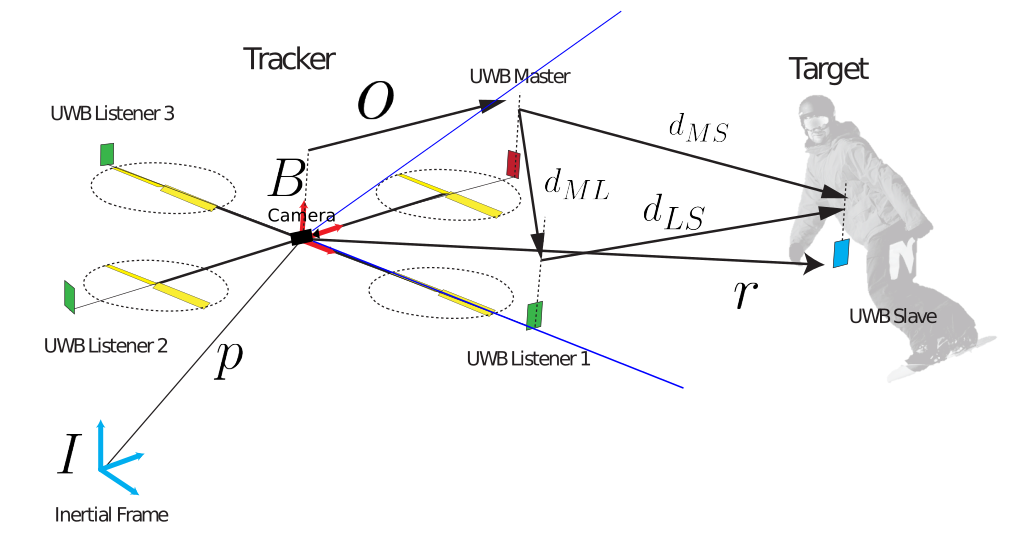
\includegraphics[height=3.5cm]{gfx/system}
	\begin{itemize}
	\item Provides 3D position information
	\item Accuracy of $\approx 10\textit{cm}$
	\end{itemize}
}

\frame{	\frametitle{Related work - Kernelized correlation filters (KCF)}
	\subsection{KCF}
	\begin{center}
	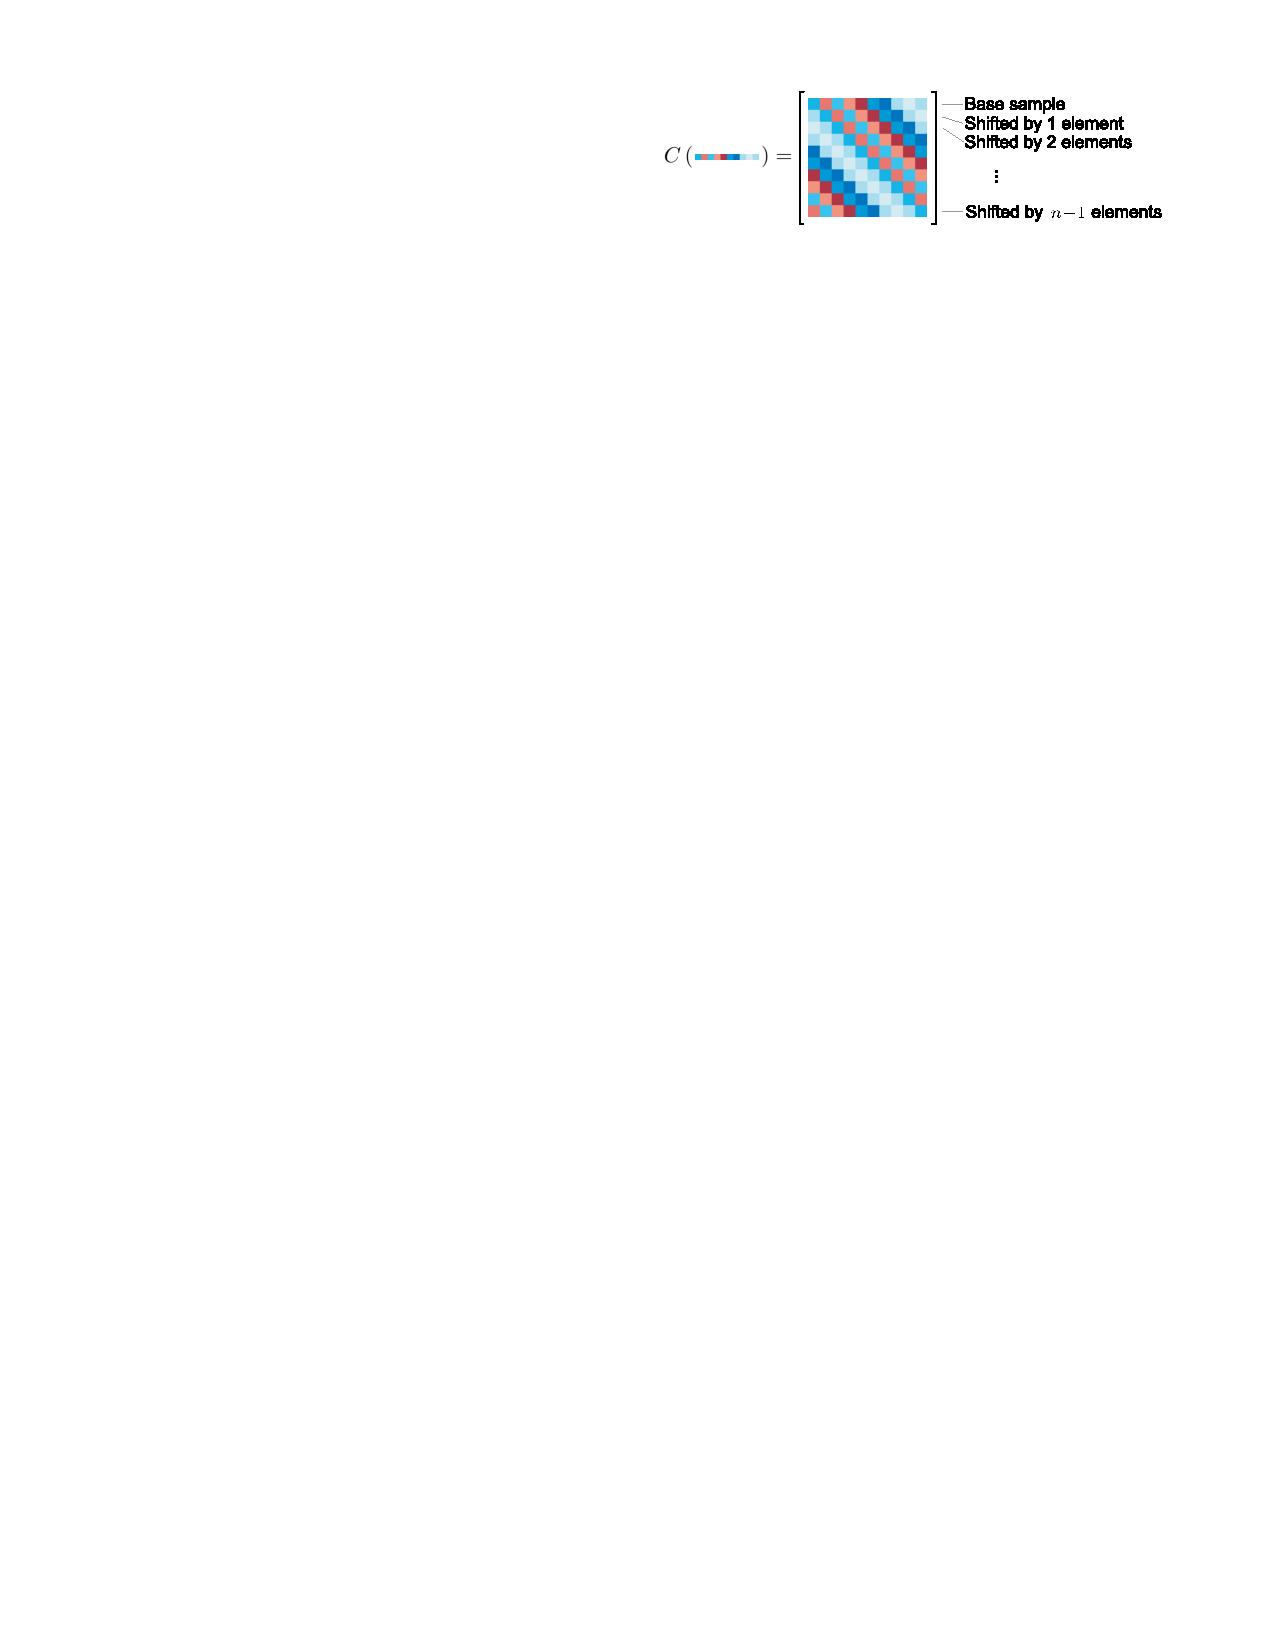
\includegraphics[width=0.5\linewidth]{gfx/circular-1}
	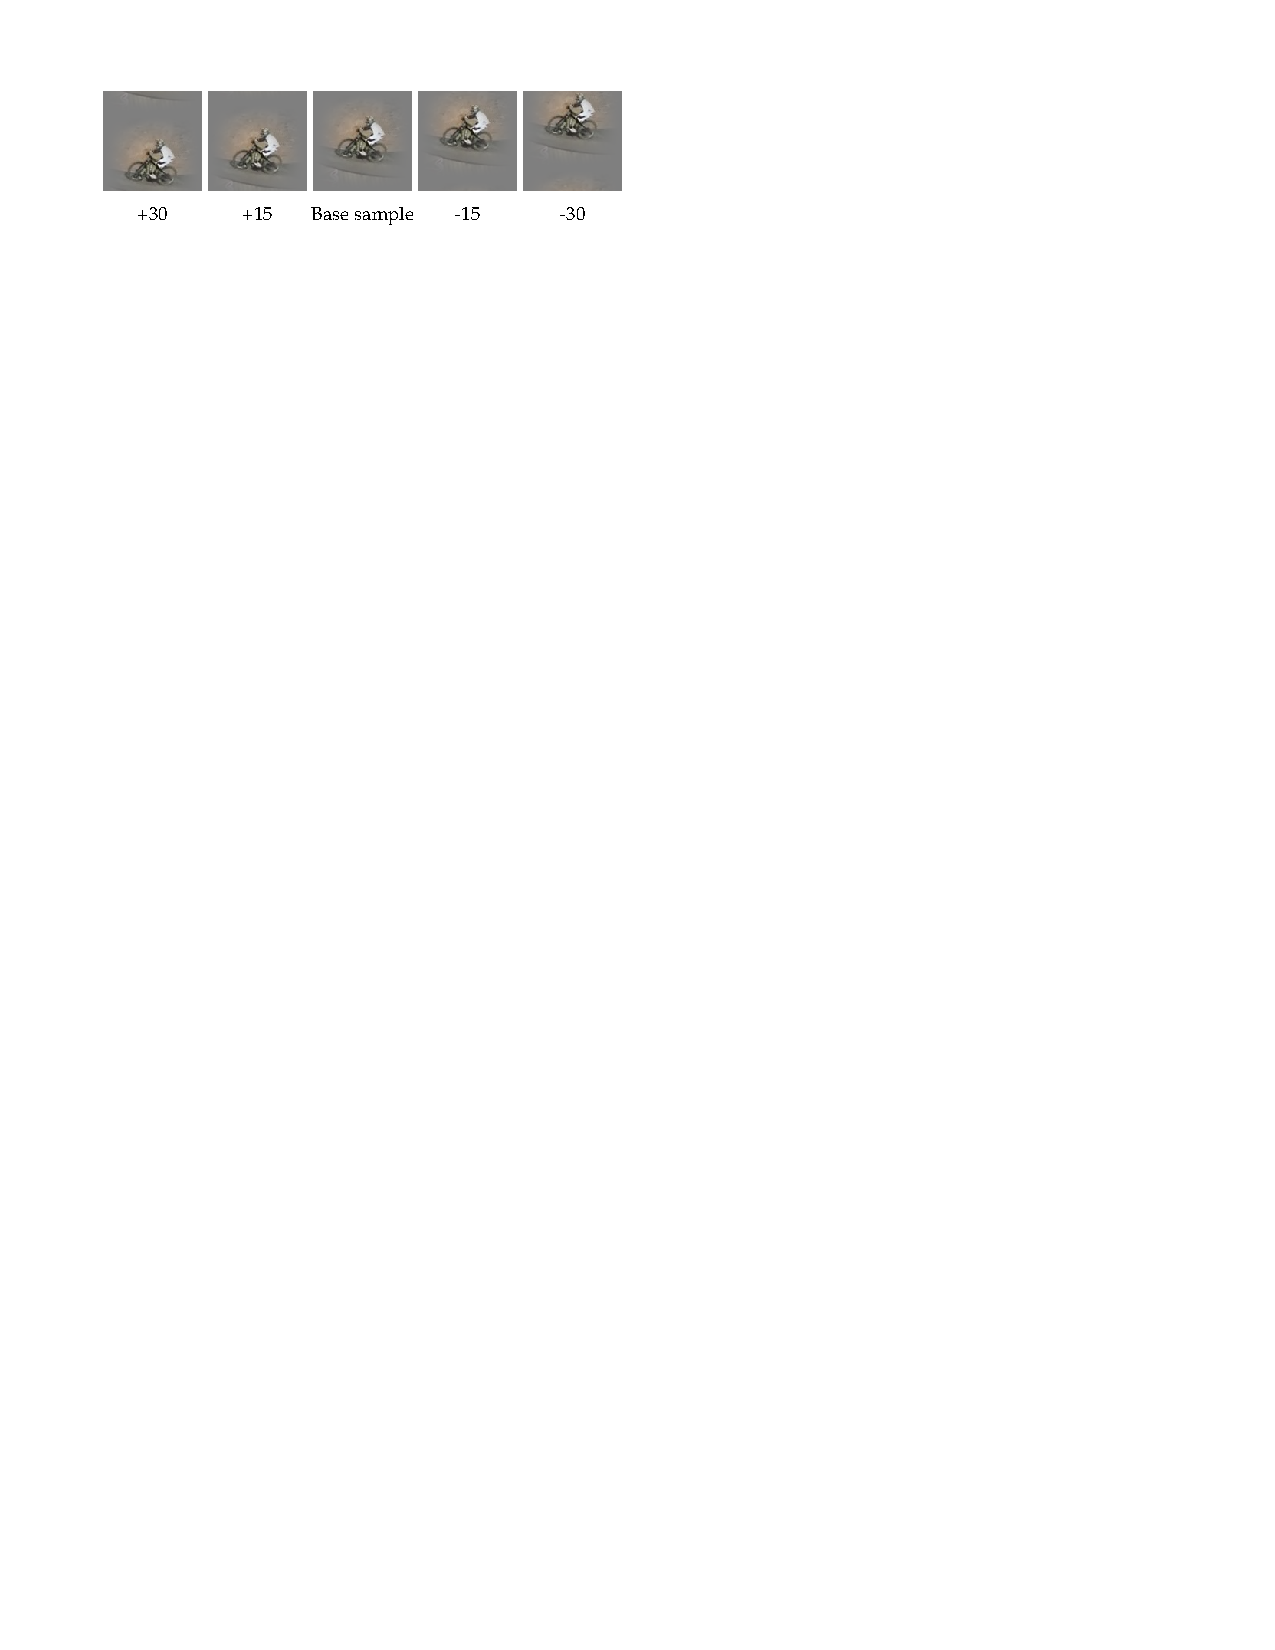
\includegraphics[width=0.5\linewidth]{gfx/circular-2}\let\thefootnote\relax\footnote{Figures from Henriques et al. 2015. High-speed tracking with kernelized correlation filters}
	\end{center}
	\begin{itemize}
	\item Translated and scaled patches are riddled with redundancies $\rightarrow$ can be represented as a circulant matrix
	\item Circulant matrices can then be diagonalized with the Discrete Fourier Transform $\rightarrow$ reduces storage as well as computation
	\item the KCF tracker can be implemented with
	only a few lines of code.
	\item 3 functions: "train", "detect" and "kernel\_correlation"
	\end{itemize}	
}

\frame{	\frametitle{Setup - Mounting}
	\section{Setup}
	\subsection{Mounting}
	\begin{itemize}
	\item Camera calibration
	\item UWB and camera mounting
	\begin{center}
	\includegraphics[height=3.0cm]{gfx/Monitor_cut}
	\end{center}
	\end{itemize}
}

\frame{	\frametitle{Setup - Matching the two coordinate systems}
	\subsection{Matching}
	\begin{itemize}
	\item ArUco \cite{Aruco2014}
	\begin{center}
	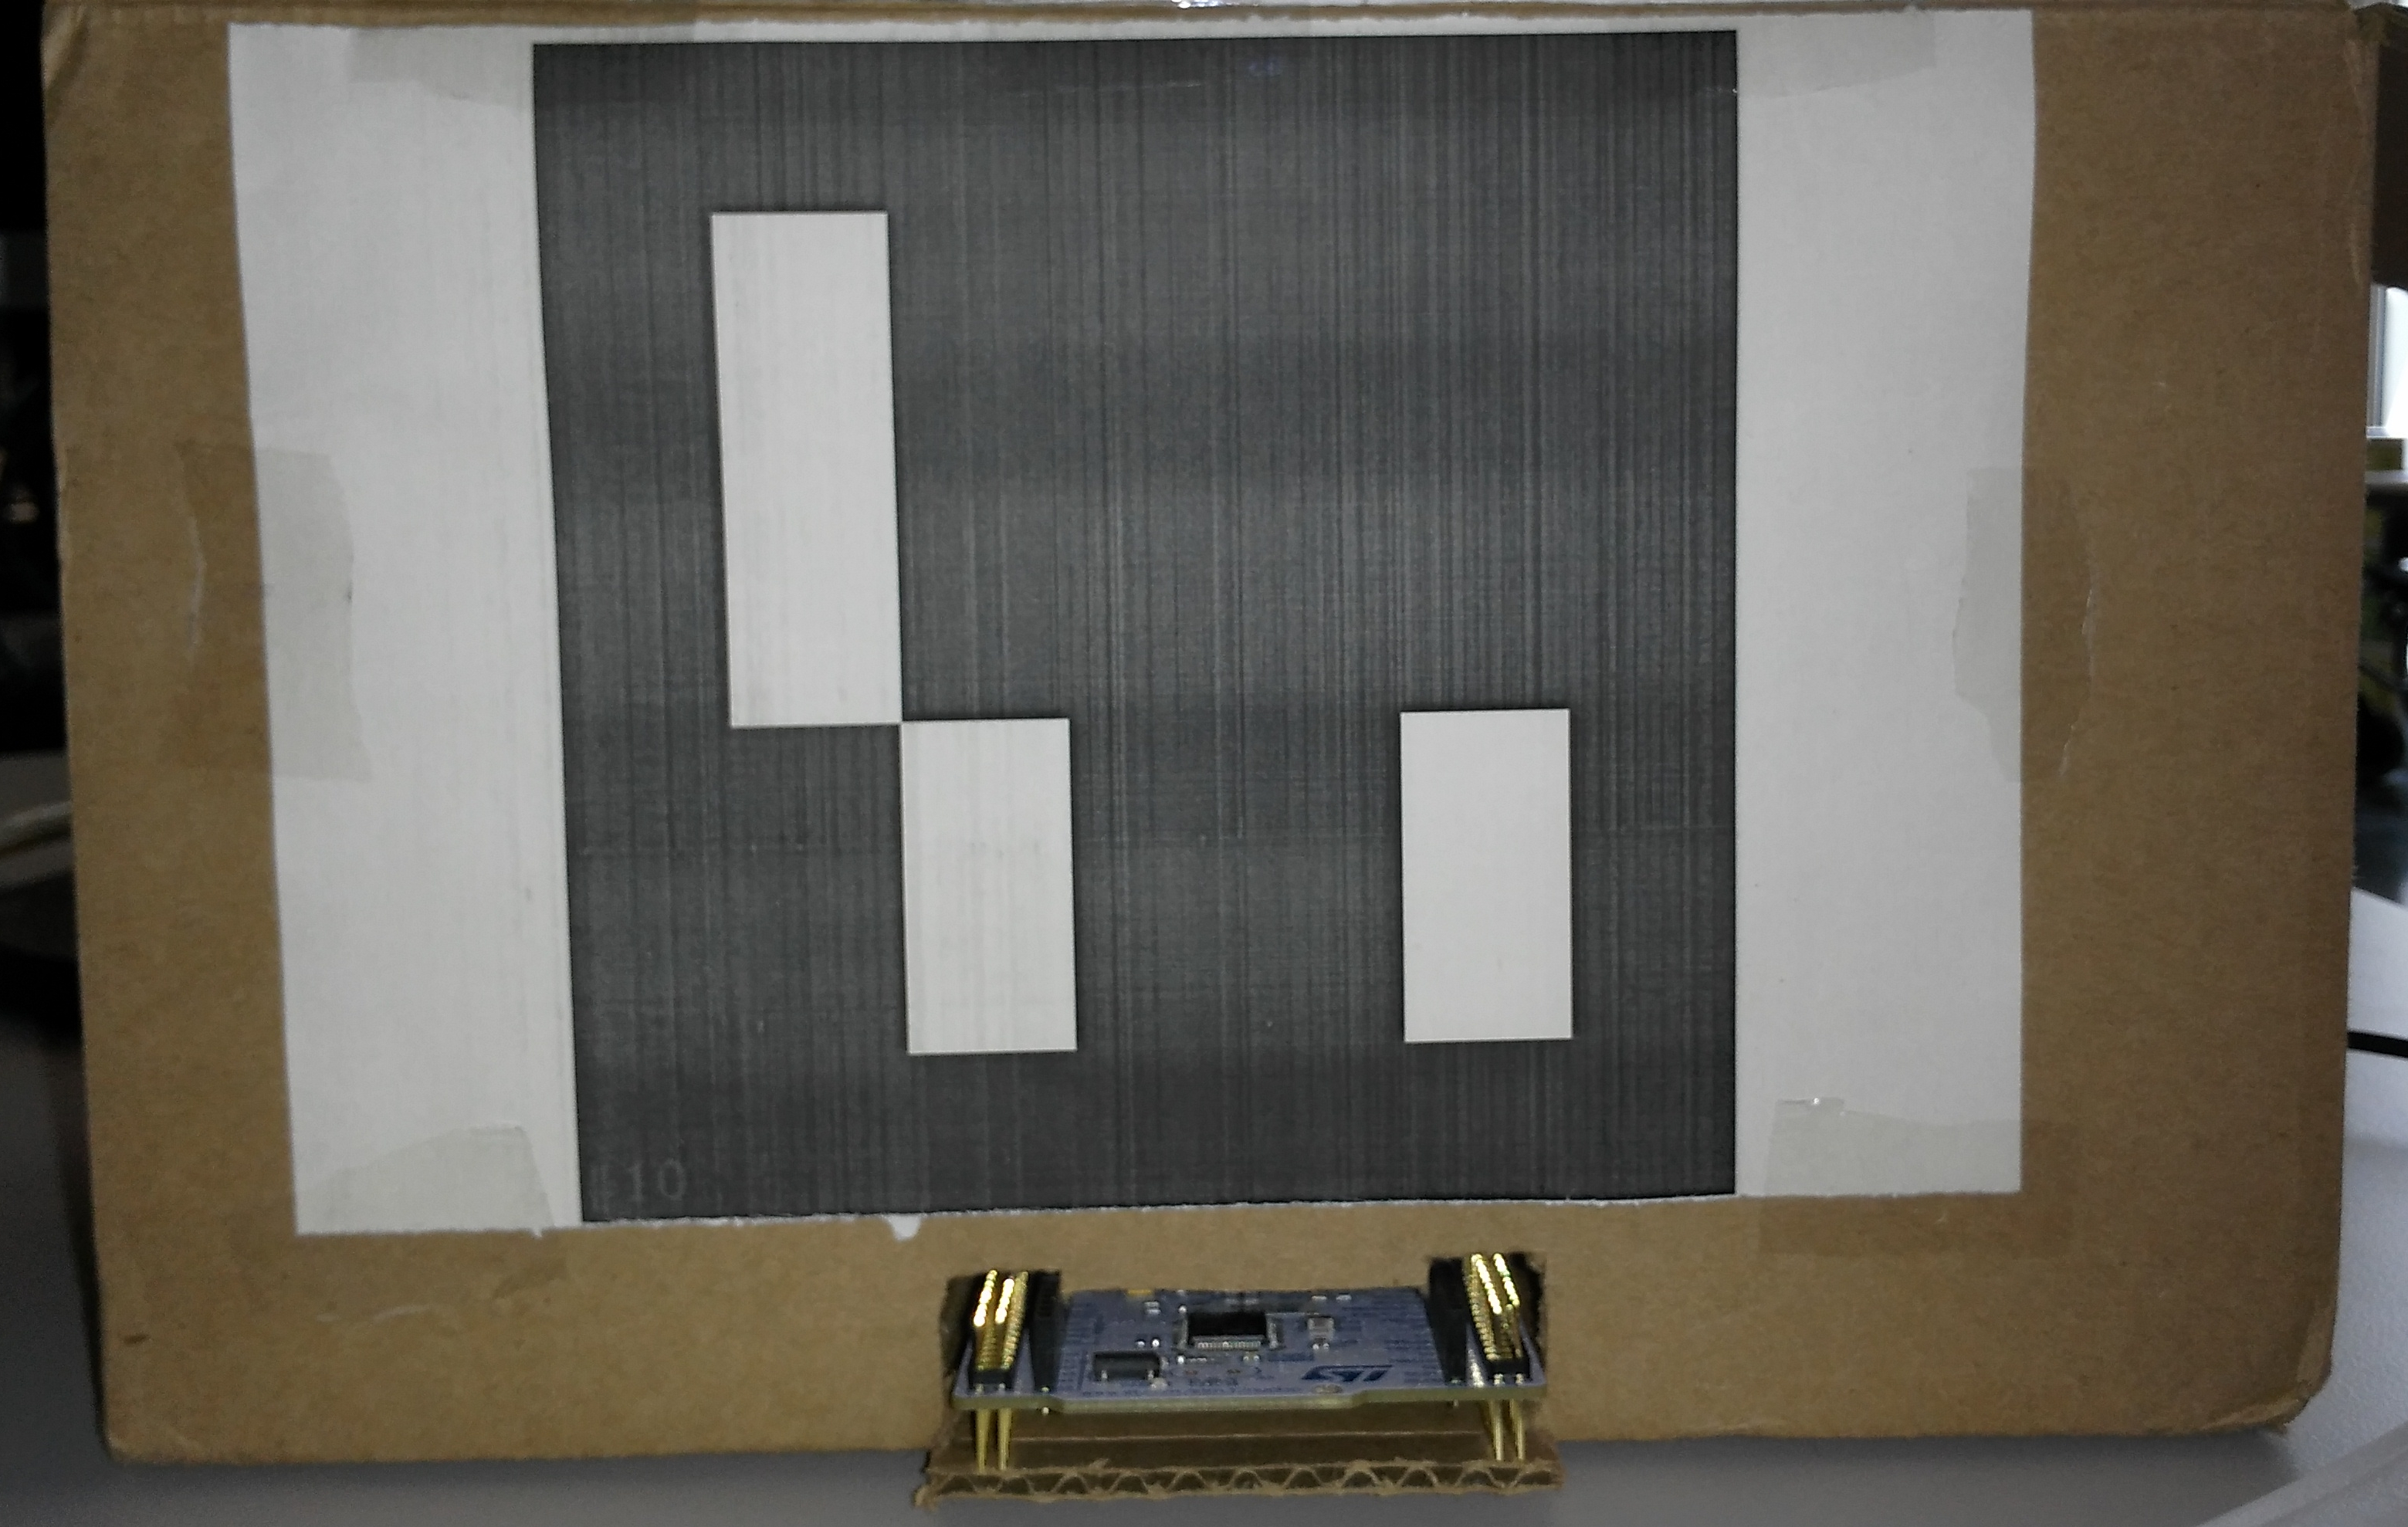
\includegraphics[height=2.0cm]{gfx/Box_cut}
	\end{center}
	\item Kabsch
	\begin{center}
	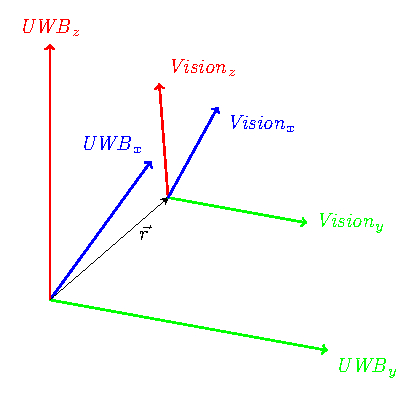
\includegraphics[height=3.0cm]{gfx/coordination_system}
	\end{center}
	\end{itemize}
}

\frame{	\frametitle{Setup - Transform between the coordinate systems}
	\subsection{Transform}
	Transform between the two coordinate systems
	\begin{center}
	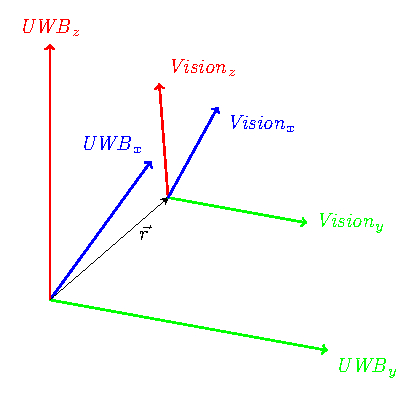
\includegraphics[height=1.5cm]{gfx/coordination_system}
	\end{center}
	Transform a point:
	\begin{equation}\label{eq:transformation}
	\begin{bmatrix}
	x_{\textit{Vision}} \\
	y_{\textit{Vision}} \\
	z_{\textit{Vision}}
	\end{bmatrix} = \frac{1}{\mathit{scale}} \cdot \textbf{U}
	\Bigg( \begin{bmatrix}
	x_{\textit{UWB}} \\
	y_{\textit{UWB}} \\
	z_{\textit{UWB}}
	\end{bmatrix} - \vec r \Bigg)
	\end{equation}
	Transform the covariance matrix:
	\begin{equation}
	\textbf{C}' = \frac{1}{\mathit{scale}^2} \textbf{U}' \textbf{C} \textbf{U}'^T
	\end{equation}
	where
	\begin{equation}
	\textbf{U}' =
	\begin{bmatrix}
	\textbf{U} & \textbf{0} \\
	\textbf{0} & \textbf{U}
	\end{bmatrix}
	\end{equation}		
}

\frame{ \frametitle{References}
	\section{References}
	\bibliography{graphics}
}

\end{document}